% mainfile: ../../../../master.tex
\subsection{Run samples on gel}
% The part of the label after the colon must match the file name. Otherwise,
% conditional compilation based on task labels does NOT work.
\label{task:20180220_cj1}
\tags{lab,dna,rna}
\authors{cj}
%\files{}
%\persons{}

\mistake{When coming in the lab, I realised that I forgot my PCR products on the bench at room temperature for more than 2 days (since Sunday) so I just throw them away.}

\subsubsection{1\% Agarose gel preparation}

\begin{enumerate}
\item Measure with erlenmeyer 75~mL of 1\% agarose gel.\sidenote{The 1\% agarose gel is kept at 60\degree C in the gel room.}
\item Warm up the erlenmeyer for 15s in microwave: agarose will be more fluid and it will avoid bubbles when casting the gel
\item Add 3.75~\textmu L of SYBR Safe to the agarose while swirling \sidenote{SYBR Safe by Invitrogen, 10,000X in \gls{dmso}}
\item Cast the gel with the comb (for 26 wells)
\comment{I used 26 wells, because the wells are smaller, and therefore the bands should be more visible.}
\item Let the gel set for 20 min
\end{enumerate}

\subsubsection{Samples preparation}

Because I do not have much material, I decided to run only 10 ng of DNA because I remembered reading that this should be enough to visualise the nucleic acids bands. So I calculate the volume of sample needed to have 10 ng of nucleic acid and I add enough loading buffer to have a total volume of 10~\uL that I can load on the gel.


\begin{itemize}
\item Transfer the calculated volume of loading buffer (with bromothymol blue) in PCR rack
\item Add the corresponding volume of each sample so the final amount of nucleic acid in each tube is 10 ng (cf. table \ref{tab:20180220_calculations_sample_on_gel})
\item Tap gently tubes to mix up everything
\item Centrifuge briefly to bring all the liquid to the bottom
\end{itemize}

\subsubsection{Electrophoresis}

For this electrophoresis migration, I run:
\begin{itemize}
\item 10~\textmu L of each sample
\item 5~\textmu L of the 1~kb ladder
\item 5~\textmu L of the 100~bp ladder
\end{itemize}

\begin{enumerate}
\item Place the agarose gel into the gel box (electrophoresis unit) containing TAE buffer
\item Load 5~\textmu L of molecular weight ladder into the first and last lane of the gel
\item Load 10~\textmu L of each sample into the additional wells of the gel
\item Run for 50~min with the \gls{eps} 301 at 100~V, 400~mA
\item Visualize your \gls{dna} fragments with \gls{uv} lights
\end{enumerate}

% latex table generated in R 3.4.3 by xtable 1.8-2 package
% Tue Feb 20 15:28:13 2018
\begin{table}[ht]
\caption{Summary of the volumes of each samples required to run nucleic acid on agarose gel}
\label{tab:20180220_calculations_sample_on_gel}
\centering
\resizebox{\textwidth}{!}{
\begin{tabular}{rlllrrrrr}
\toprule 
Nucleic & \multirow{2}{*}{Label} & Extraction & Quantification & Concentration & Volume & Amount & Volume & Volume of \\ 
acid &  & kit & assay & (ng/\uL) & (\uL) & (ng) & for gel (\uL) & loading buffer (\uL) \\ 
\midrule
\multirow{4}{*}{DNA} & \texttt{MP1} & MasterPure\texttrademark~ & Qubit\texttrademark~ dsDNA BR & 3.11 & 50.00 & 155.50 & 3.22 & 6.78 \\ 
   & \texttt{AP1} & AllPrep & Qubit\texttrademark~ dsDNA BR & 2.44 & 100.00 & 244.00 & 4.10 & 5.90 \\ 
   & \texttt{AP2} & AllPrep & Qubit\texttrademark~ dsDNA BR & 5.86 & 150.00 & 879.00 & 1.71 & 8.29 \\ 
   & \texttt{MP2} & MasterPure\texttrademark & Qubit\texttrademark~ dsDNA BR & 18.20 & 50.00 & 910.00 & 0.55 & 9.45 \\ 
   \midrule
  \multirow{4}{*}{RNA} & 
 \texttt{MP1} & MasterPure & Qubit\texttrademark~ RNA BR & 7.20 & 50.00 & 360.00 & 1.39 & 8.61 \\ 
   & \texttt{AP1} & AllPrep & Qubit\texttrademark~ RNA BR & 8.77 & 50.00 & 438.50 & 1.14 & 8.86 \\ 
   & \texttt{AP2} & AllPrep & Qubit\texttrademark~ RNA BR & 31.50 & 80.00 & 2520.00 & 0.32 & 9.68 \\ 
   & \texttt{MP2} & MasterPure\texttrademark & Qubit\texttrademark~ RNA BR & 32.20 & 50.00 & 1610.00 & 0.31 & 9.69 \\ 
\bottomrule 
\end{tabular}
}
\end{table}

\begin{figure}[H] % position of the figure 
    \centering
    \caption{Picture of 1\% agarose gel after 50 minute-long electrophoresis migration of 10~ng DNA and RNA samples extracted from micro-algae cultures with MasterPure\texttrademark~ or AllPrep kits.}
    \label{fig:20180220_DNA_RNA_MP_vs_AP_10ng}
    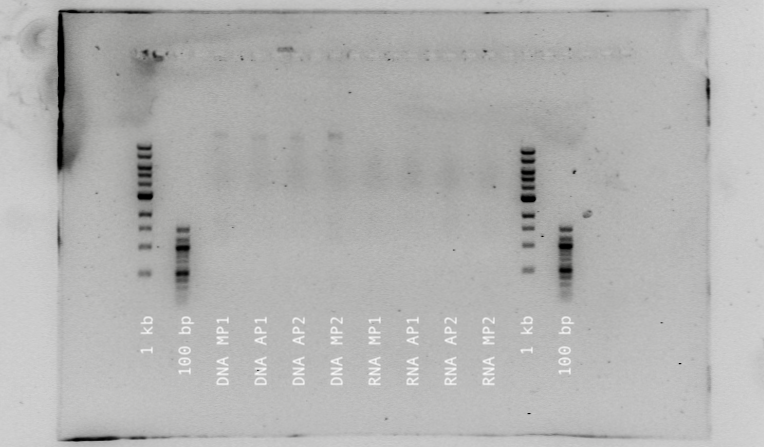
\includegraphics[width=\textwidth]{graphics/pic/20180220_DNA_RNA_MP_vs_AP_10ng.png}
\end{figure}

On the gel shown in figure \ref{fig:20180220_DNA_RNA_MP_vs_AP_10ng}, we can see the four samples of DNA but the RNA is not visible which makes sense because I used SYBR Safe stain which stains DNA but not RNA.

\sidenote{\url{https://www.researchgate.net/post/Running_a_genomic_DNA_quality_check_on_a_gel-can_anyone_help}}
\sidenote{\url{https://www.researchgate.net/post/What_is_the_minimum_DNA_quantity_ng_required_to_visualize_DNA_on_Agarose_gel}}

After further reading on ResearchGate, I will try again to run the DNA samples ona gel tomorrow. Because the concentrations of DNA in my samples are very variable I will not be able to run 50 ng of DNA for all samples. So I think I can try to run 5~\uL of each samples (with 5~\uL of loading buffer) and see if I can see more details. I can also discuss this with Viggó tomorrow.
